%% 18.022 cheat sheet
%%
%% Copyright (C) 2009, 2010, 2011 Benjamin Barenblat
%%                                http://benjamin.barenblat.name/
%%
%% This document is licensed under the Creative Commons
%% Attribution-NonCommercial-ShareAlike 3.0 United States License.
%% For more information, see
%% http://creativecommons.org/licenses/by-nc-sa/3.0/us/.
%%
%% This document is designed to be typeset with pdfLaTeX.
\documentclass[10pt,landscape]{article}
\usepackage{eco}
\usepackage{geometry}
\usepackage{multicol}
\usepackage{mathtools}
\usepackage{color}
\usepackage[colorlinks]{hyperref}
\definecolor{darkred}{rgb}{0.5,0,0}
\hypersetup{colorlinks,linkcolor=black,urlcolor=darkred}
\usepackage{graphicx}
\usepackage{wrapfig}
\usepackage{18.022}
\usepackage{esint}
\usepackage{titlesec}

% Only show equation numbers of referenced equations.
\mathtoolsset{showonlyrefs=true}

% Set margin.
\geometry{margin=6mm}

% Turn off header and footer.
\pagestyle{empty}

% Don't print subsection numbers.
\setcounter{secnumdepth}{0}

%% Squash paragraph headings.
\titlespacing*{\paragraph}{0pt}{.94em}{*1}

\setlength{\parindent}{0pt}
\setlength{\parskip}{0pt}

\makeatletter
\newcommand{\@recitation}{}
\newcommand{\recitation}[1]{\renewcommand{\@recitation}{#1}}
\renewcommand{\maketitle}{%
  \begin{center}
    \LARGE{\textbf{\@title}}
  \end{center}
}
\newcommand{\makeend}{%
  \vfill
  \rule{0.3\linewidth}{0.25pt}
  \scriptsize
  \begin{tabular}{@{}l}
    Copyright \copyright\ \@date\ \@author.  \href{http://creativecommons.org/licenses/by-nc-sa/3.0/us/}{\textsc{cc by$\cdot$nc$\cdot$sa}}.  No warranty.\\
    \url{http://benjamin.barenblat.name/}
  \end{tabular}
}
\makeatother

\title{18.022 Cheat Sheet}
\author{Benjamin Barenblat}
\date{2009--2011}

\begin{document}
\raggedright
\begin{multicols*}{3}
\maketitle

\section{Vectors}
\paragraph{Dot product}
Let $\vec v, \vec w, \vec u \in \R^n$.
Then, $\vec v \dot \vec w = \langle \vec v, \vec w \rangle = \langle\vec v \vert \vec w\rangle = \bra v_1w_1 & \cdots & v_nw_n \ket$.

\paragraph{Cauchy-Schwarz inequality}
Let $\vec v, \vec w \in \R^n$.
Then, $(\vec v \dot \vec w)^2 \le (\vec v \dot \vec v)(\vec w \dot \vec w) \iff \abs{\vec v \dot \vec w} \le \norm{\vec v}\norm{\vec w}$.

\paragraph{Triangle inequality}
Let $\vec v, \vec w \in \R^n$.
Then, $\norm{\vec v + \vec w} \le \norm{\vec x} + \norm{\vec y}$ and $\norm{\vec v - \vec w} \ge \big\lvert\norm{\vec v} - \norm{\vec w}\big\rvert$.

\paragraph{Projection}
For $\vec a, \vec b \in \R^n$, the projection of $\vec b$ onto $\vec a$
\begin{equation}
  \label{eq:projection}
  \proj_{\vec a}\vec b = \frac{\vec a \dot \vec b}{\norm{\vec a}}\vec{\hat a} = \frac{\vec a \dot \vec b}{\norm{\vec a}^2}\vec a = \frac{\vec a \dot \vec b}{\vec a \dot \vec a}\vec a
\end{equation}
and $\norm{\proj_{\vec a}\vec b} = \norm{\vec b\cos\theta}$.

\paragraph{Distance from a point to a line}
Given a point $\vec p$ and a line $\vec l(t) = \vec vt + \vec q$, the shortest vector from $\vec p$ to $\vec l$ is
\begin{equation}
  \vec q - \vec p - \proj_{\vec v}(\vec q - \vec p) = \vec q - \vec p - \frac{(\vec q - \vec p) \dot \vec v}{\norm{\vec q - \vec p}^2}\vec v.
\end{equation}

\paragraph{Cross product}
Let $\vec v, \vec w \in \R^3$.
Then,
\begin{equation}
  \label{eq:crossproduct}
  \vec v \cross \vec w = \bra v_1 \\ v_2 \\ v_3 \ket \cross \bra w_1 \\ w_2 \\ w_3 \ket = \bra v_2w_3 - v_3w_2 \\ v_3w_1 - v_1w_3 \\ v_1w_2 - v_2w_1 \ket
\end{equation}
and
$\norm{\vec v \cross \vec w} = \norm{\vec v}\norm{\vec w}\abs{\sin\theta}$.

\paragraph{Planes}
Let $\vec x = \bra x_1 & \cdots & x_n \ket \in \R^n$.
For a point $\vec p$ and normal vector $\vec n$, $(\vec x - \vec p) \dot \vec n = 0$.
\begin{list}{\textbullet}{\setlength{\itemsep}{0pt}}
\item Point and two vectors: $\vec n = \vec u \cross \vec v$.
\item Three points: $\vec n = (\vec q - \vec p) \cross (\vec r - \vec p) = 0$.
\item Function and point: $\vec n = \grad f(\vec p)$.
\end{list}

\paragraph{Triple scalar product / determinant}
For $\vec u, \vec v, \vec w \in \R^3$,
\begin{equation}
  \vec u \dot \vec v \cross \vec w = \det \bra \vec u & \vec v & \vec w \ket
\end{equation}
is the volume of the parallelepiped spanned by $\vec u$, $\vec v$, and $\vec w$.
$(\vec u, \vec v, \vec w)$ is right-handed iff $\det \bra \vec u & \vec v & \vec w \ket > 0$.

\paragraph{Matrix Multiplication}
Dimensionally, the number of columns in the first matrix must match the number of rows in the second.
\begin{wrapfigure}[5]{r}{1.4in}
  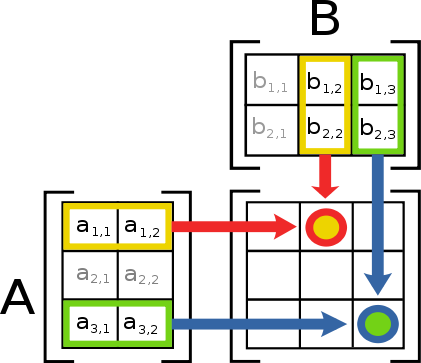
\includegraphics[width=1.4in]{matrix-multiplication}
  \scriptsize Copyright \textcopyright\ 2009 \href{http://en.wikipedia.org/wiki/User:Fangfufu}{Fangfufu}.\\\textsc{\href{http://creativecommons.org/licenses/by-sa/3.0/}{cc by$\cdot$sa}}.
\end{wrapfigure}
\begin{multline}
  \bra a & b & c \\ d & e & f \\ g & h & i \ket \bra \alpha & \delta \\ \beta & \epsilon \\ \gamma & \zeta \ket = \\ \bra a\alpha + b\beta + c\gamma & a\delta + b\epsilon + c\zeta \\ d\alpha + e\beta + f\gamma & d\delta + e\epsilon + f\zeta \\ g\alpha + h\beta + i\gamma & g\delta + h\epsilon + i\zeta\ket
\end{multline}
$a_{1,2}$ refers to the element in the $1$st row, $2$nd column.
Generally, for two matrices $A$ and $B$,
\begin{equation}
  (AB)_{i,j} = A_{i,1} + B_{1,j} + A_{i,2}B{2,j} + \cdots + A_{i,n}B_{n,j}.
\end{equation}

\section{Differential calculus}
\paragraph{Gradient}
For a scalar field $f : \R^n \to \R$, the gradient of $f$
\begin{equation}
  \grad f = \bra D_1f \\ D_2f \\ D_3f \\ \vdots \\ D_nf \ket,
\end{equation}
a new vector field which consistently points in the direction of $f$'s greatest increase with magnitude equal to the rate of that increase.
By corollary, $\grad f$ is always perpendicular to $f$'s level curves.

\paragraph{Divergence}
For a vector field $\vec F : \R^n \to \R^n$, the divergence of $\vec F$
\begin{equation}
  \div\vec F = D_1F_1 + D_2F_2 + D_3F_3 + \cdots + D_nF_n,
\end{equation}
a new scalar field.
Positive values of $\div\vec F$ indicate field sources, while negative values indicate field sinks.

\paragraph{Curl}
For a vector field $\vec F : \R^3 \to \R^3$, the curl of $\vec F$
\begin{equation}
  \curl\vec F = \bra D_2F_3 - D_3F_2 \\ D_3F_1 - D_1F_3 \\ D_1F_2 - D_2F_1 \ket,
\end{equation}
a new vector field measuring the rate of rotation at each point.

\paragraph{Laplacian}
For a scalar field $f : \R^n \to \R$, the Laplacian of $f$
\begin{equation}
  \nabla^2 f = \div\grad f = D_1^2f + D_2^2f + D_3^2f + \cdots + D_n^2f.
\end{equation}

\paragraph{Conservative vector fields}
Let $\vec F : U \subseteq \R^n \to \R^n$ ($U$ open) be a vector field
of class $C^1$.  If there exists a class $C^2$ scalar field $f : U \to
\R$ such that $\vec F = \grad f$ on $U$, then $\vec F$ is conservative
on $U$.  If $\vec F$ is conservative on $U$, then $\vec F$ is also
curl-free on $U$.  (The converses are true if $U$ is simply connected.)

\paragraph{Chain rule}
If $\vec f : \R^n \to \R^m$ is differentiable at $\vec x$ and $\vec g
: \R^m \to \R^p$ is differentiable at $\vec f(\vec x)$, then $\vec g
\circ \vec f$ is differentiable at $\vec x$ and
\begin{equation}
  \label{eq:chainrule}
  D(\vec g \circ \vec f)_{\vec x} = \big(D\vec g_{\vec f(\vec x)}\big)(D\vec f_{\vec x}).
\end{equation}

\paragraph{Implicit function theorem}
Let $\vec F : \R^{n+m} \to \R^m$ (i.e., $m$ functions in $n + m$ unknowns) be of class $C^1$ and let $\vec F(\vec x_0) = \0$ for some $\vec x_0 \in \R^{n+m}$.
Write $\vec x = (\vec a, \vec b)$, where $\vec a \in \R^n$ and $\vec b \in \R^m$; write $\vec x_0 = (\vec a_0, \vec b_0)$, where $\vec a_0 \in \R^n$ and $\vec b_0 \in \R^m$.
Note that $D\vec F = \bra D_{\vec a}\vec F & D_{\vec b}\vec F \ket$.
If $D_{\vec b}\vec F(\vec b_0)$ is invertible (i.e., $\det D_{\vec b}\vec F(\vec b_0) \ne 0$), then there exists a neighborhood $U$ of $\vec a_0$ in $\R^n$ and a neighborhood $V$ of $\vec b_0$ in $\R^m$ and a function $\vec f : U \to V$ such that $F\big(\vec a_0, f(\vec a_0)\big) = 0$.
$\vec f$ expresses $\vec b$ in terms of $\vec a$ in the neighborhood of $(\vec a_0, \vec b_0)$, and
\begin{equation}
  \label{eq:implicitdiff}
  D\vec f_{\vec a_0} = -\big(D_{\vec b}\vec F(\vec b_0)\big)^{-1}\big(D_{\vec a}\vec F(\vec a_0)\big).
\end{equation}

\paragraph{Taylor's theorem}
The $k$th-order Taylor polynomial of a class $C^k$ function $f : \R^2 \to \R$ at $\vec x \in \R^2$ near a point $\vec a \in \R^2$
\begin{equation}
  T^kf_{\vec a}(\vec x - \vec a) = \sum_{\substack{n,m\\n+m \le k}} \frac{D_1^nD_2^m f(a_1,a_2)}{n!m!}(x - a_1)^n(y - a_2)^m.
\end{equation}

\paragraph{Extrema}
Consider a function $f : \R^n \to \R$ of class $C^2$.
$f$ has critical points where $Df = \0$; if $f$ has local extrema, they will occur at critical points.
At each critical point,
\begin{itemize}
\item If $D^2f$'s minors are all positive, $D^2f$ is positive definite and the point is a local minimum.
\item If $-D^2f$'s minors are all positive, $D^2f$ is negative definite and the point is a local maximum.
\item If neither of these are true, but $D^2f$ is invertible, $D^2f$ is indefinite and the point is a saddle point.
\item If $D^2f$ is not invertible, then the point is degenerate.
\end{itemize}
If a function $f : K \to \R$ is of class $C^1$ on $K$ and continuous on the interior of $\partial K$ and $K$ is closed and bounded, then $f$ has at least one minimum and at least one maximum on $K$.
The extrema will occur inside $K$ at critical points or somewhere on $\partial K$.

\paragraph{Constrained optimization (one constraint)}
Consider a differentiable function $f : \R^n \to \R$ on a set $\mathscr{C} \subseteq \R$ defined as the level set of some function -- i.e., for some $C^1$ function $g$, $\mathscr{C} = \{ \vec x \in \R^n : g(\vec x) = 0 \}$.
Define $L(\vec x, \lambda) = f(\vec x) - \lambda g(\vec x)$.
If, at a point $\vec x_0$, $\grad L(\vec x_0, \lambda_0) = 0$ for some constant $\lambda_0$ and $\grad g(\vec x_0) \ne 0$, then $f\vert_\mathscr{C}$ has a critical point at $\vec x_0$.

\paragraph{Constrained optimization ($k$ constraints)}
Consider a differentiable function $f : \R^n \to \R$ on a set $\mathscr{C} \subseteq \R$ defined as the level set of some family of functions -- i.e., for some $C^1$ function $\vec g = \bra g_1 & g_2 & \cdots & g_n \ket$, $\mathscr{C} = \{ \vec x \in \R^n : \vec g(\vec x) = \0 \}$.
Define $L(\vec x, \boldsymbol\lambda) = f(\vec x) - \boldsymbol\lambda \dot \vec g(\vec x)$.
If, at a point $\vec x_0$, $\grad L(\vec x_0, \boldsymbol\lambda_0) = 0$ for some constant $\boldsymbol\lambda_0$ and $\bra \grad g_1(\vec x_0) & \cdots & \grad g_k(\vec x_0) \ket$ has a $k\times k$ submatrix that is invertible, then $f\vert_\mathscr{C}$ has a critical point at $\vec x_0$.

\section{Integral calculus}
\paragraph{Double integrals}
Let $f : \R^2 \to \R$ be Riemann integrable on some nice domain $D \subseteq \R^2$.
Define $a, b, c, d \in \R$ such that $[a,b] \times [c,d]$ is $D$'s bounding box.
Now define $f$'s extension
\begin{equation}
  f^{\text{ext}}(x,y,z) = \begin{cases}
    f(x,y) & \text{if $(x,y) \in D$},\\
    0 & \text{otherwise}.
    \end{cases}
\end{equation}
Then,
\begin{equation}
  \iint_D f(x,y) dxdy = \int_a^b \int_c^d f^{\text{ext}}(x,y) dydx.
\end{equation}
In practice,
\begin{equation}
  \iint_D f(x,y) dxdy = \int_a^b \int_{g(x)}^{h(x)} f^{\text{ext}}(x,y) dydx
\end{equation}j
for some functions $g$ and $h$.

\paragraph{Triple integrals}
Let $f : \R^3 \to \R$ be Riemann integrable on some nice domain $D \subseteq \R^3$.
Define $a, b, c, d, e, f \in \R$ such that $[a,b] \times [c,d] \times [e,f]$ is $D$'s bounding box.
Now define $f$'s extension
\begin{equation}
  f^{\text{ext}}(x,y,z) = \begin{cases}
    f(x,y,z) & \text{if $(x,y,z) \in D$},\\
    0 & \text{otherwise}.
    \end{cases}
\end{equation}
Then,
\begin{equation}
  \iiint_D f(x,y,z) dxdydz = \int_a^b \int_c^d \int_e^f f^{\text{ext}}(x,y,z) dzdydx.
\end{equation}
In practice,
\begin{multline}
  \iiint_D f(x,y,z) dxdydz\\ = \int_a^b \int_{g(x)}^{h(x)} \int_{p(x,y)}^{q(x,y)} f^{\text{ext}}(x,y,z) dzdydx
\end{multline}
for some functions $g$, $h$, $p$, and $q$.

\paragraph{Change of variables}
Let $f : D \subset \R^n \to \R$ be Riemann integrable on some nasty domain $D$ and let $\boldsymbol\Phi : D^* \subset \R^n \to D$ be such that $\boldsymbol\Phi$ is of class $C^1$, $\boldsymbol\Phi$ is one-to-one, $\boldsymbol\Phi$ is invertible on its domain (i.e., $\det D\boldsymbol\Phi_{\vec u} \ne 0$ for all $\vec u \in D^*$), and $\boldsymbol\Phi(D^*) = D$.  Then,
\begin{equation}
  \int_D f(\vec x) d\vec x = \int_{D^*} f\big(\boldsymbol\Phi(\vec u)\big)\abs{\det D\boldsymbol\Phi_{\vec u}} d\vec u.
\end{equation}
For well-known coordinate systems, $dxdy = rdrd\theta$; $dxdydz = \rho^2\sin\phi d\rho d\phi d\theta = rdrd\theta dz$.

\paragraph{Scalar line integrals}
Let $\vec x(t) : \R \to \R^n$ parametrize a curve $C$ in $\R^n$ with endpoints $\vec x(a)$ and $\vec x(b)$; let $f(\vec x) : \R^n \to \R$ be a function defined on $C$.
Then,
\begin{equation}
  \int_C fds = \int_a^b f\big(\vec x(t)\big) \norm{\vec{\flux x}(t)} dt.
\end{equation}

\paragraph{Vector line integrals}
Let $\vec x(t) : \R \to \R^n$ parametrize a curve $C$ in $\R^n$ with endpoints $\vec x(a)$ and $\vec x(b)$; let $\vec F(\vec x) : \R^n \to \R^m$ be a vector field defined on $C$.
Then,
\begin{equation}
  \int_C \vec F \dot d\vec s = \int_a^b \vec F\big(\vec x(t)\big) \dot \vec{\flux x}(t) dt.
\end{equation}

\paragraph{Scalar surface integrals}
Let $\vec X(u,v) : \R^2 \to \R^n$ be a piecewise smooth parametrization of a surface $\mathscr{S}$ in $\R^n$ such that $\vec X(D) = \mathscr{S}$; let $f(\vec X) : \R^n \to \R$ be a function defined on $\mathscr{S}$.
Then,
\begin{equation}
  \iint_\mathscr{S} fdS = \iint_D f\big(\vec X(u,v)\big) \norm{\frac{\partial\vec X}{\partial u} \cross \frac{\partial\vec X}{\partial v}} dudv.
\end{equation}

\paragraph{Vector surface integrals}
Let $\vec X(u,v) : \R^2 \to \R^n$ be a piecewise smooth parametrization of a surface $\mathscr{S}$ in $\R^n$ such that $\vec X(D) = \mathscr{S}$; let $\vec F(\vec X) : \R^n \to \R^m$ be a vector field defined on $\mathscr{S}$.
Then,
\begin{equation}
  \iint_\mathscr{S} \vec F \dot d\vec S = \iint_D \vec F\big(\vec X(u,v)\big) \dot \frac{\partial\vec X}{\partial u} \cross \frac{\partial\vec X}{\partial v} dudv.
\end{equation}
The first member of this definition, $\iint_\mathscr{S} \vec F \dot d\vec S$, is also called the flux of $\vec F$ through $\mathscr{S}$.

\section{Fundamental theorems}
\paragraph{The first fundamental theorem of calculus}
If $f : \R^n \to \R$ is of class $C^1$ and $C$ is a smooth curve in $\R^n$ with endpoints $\vec x_0$ and $\vec x_1$, then
\begin{equation}
  \int_C \grad f \dot d\vec s = f(\vec x_1) - f(\vec x_0).
\end{equation}

\paragraph{Green's theorem}
Let $D$ be a closed set in $\R^2$ such that $\partial D$ is a collection of closed curves oriented such that $D$ is to the left.
If $\vec F: D \to \R^2$ is of class $C^1$, then
\begin{equation}
  \oint_{\partial D} \vec F \dot d\vec s = \iint_D \curl \vec F \dot \vec k dxdy.
\end{equation}
This is a special case of Stokes' theorem.

\paragraph{Gauss's theorem (the second fundamental theorem of calculus)}
Let $\Omega \in \R^3$ be a closed domain whose boundary is a piecewise smooth surface $\partial\Omega$.
Give $\partial\Omega$ outward-pointing orientation.
If $\vec F$ is a $C^1$ vector field in $\Omega$, then
\begin{equation}
  \oiint_{\partial\Omega} \vec F \dot d\vec S = \iiint_\Omega \div\vec F dxdydz.
\end{equation}

\paragraph{Stokes' theorem (the third fundamental theorem of calculus)}
Let $\mathscr{S}$ be a piecewise smooth surface in $\R^3$ with a given continuous normal vector field $\vec N$.
Let $\partial\mathscr{S}$ be a collection of piecewise smooth curves.
Orient the curves such that the outside of the surface is to the left.
Now let $\vec F : \mathscr{S} \to \R$ be a $C^1$ vector field.
Then,
\begin{equation}
  \oint_{\partial\mathscr{S}} \vec F \dot d\vec s = \iint_\mathscr{S} \curl \vec F \dot d\vec S.
\end{equation}

\makeend
\end{multicols*}
\end{document}
